\section*{Введение}
\addcontentsline{toc}{section}{Введение}
\lipsum[1-3]
\newpage



\section{Анализ технического задания}
\subsection{Постановка задачи}
\lipsum[4]

Пример библиографической ссылки~\cite{wiki_main}.
Пример нумерации:
\begin{enumerate}
\item пункт1;
\item пункт2;
\item пункт3;
\item пункт4;
\item пункт5;
\item пункт6;
\item пункт7.
\end{enumerate}

\lipsum[5]
\begin{itemize}
\item пункт1;
\item пункт2;
\item пункт3;
\item пункт4;
\item пункт5;
\item пункт6;
\item пункт7.
\end{itemize}

\subsection{Назначение разрабатываемого программного продукта}
\lipsum[6]

\subsection{Анализ исходных данных к курсовой работе}
\lipsum[7]

\subsection{Методы и алгоритмы решения задачи}
\lipsum[34]

\subsection{Требования к разработке}
\lipsum[38]
\newpage



\section{Разработка математической модели}
\lipsum[40]
\newpage



\section{Разработка алгоритмов работы системы}
\subsection{пункт1}
\lipsum[9]

\subsection{пункт2}
\lipsum[10]

\subsubsection{под под пункт 1}
\lipsum[11]

\subsubsection{под под пункт 2}
\lipsum[12]
\newpage



\section{Разработка программной системы}
\subsection{пункт 1}
\lipsum[52]

\subsection{пункт 2}
Пример вставки исходного кода "как есть".


\lipsum[13]
\newpage



\section{Руководство по программному продукту}
\subsection{Руководство программиста}
Структура проекта представлена на рисунке~\ref{fig:structure} (пример вставки рисунка).

\begin{figure}[b]
\centering
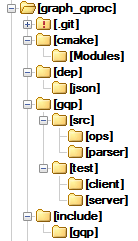
\includegraphics[scale=1]{structure}
\caption{Дерево файлов проекта}
\label{fig:structure}
\end{figure}

\lipsum[14-16]

\subsection{Руководство администратора}
\lipsum[17]

\subsection{Руководство пользователя}
\lipsum[18-19]
\newpage



\section{Тестирование системы}
\lipsum[19-21]
\newpage



\section*{Заключение}
%\addtocontents{toc}{\protect\newpage}
\addcontentsline{toc}{section}{Заключение}
\lipsum[23-25]